\documentclass[a4paper, oneside, 11pt]{article}
\usepackage{amssymb}
\usepackage{amsmath}
\usepackage{amsfonts}
\usepackage{amsthm}
\usepackage{graphicx,rotating,booktabs}
\usepackage[verbose]{placeins}
\usepackage[latin1]{inputenc}
\usepackage[T1]{fontenc}
\usepackage{graphicx}
\usepackage{caption}
\usepackage{tabularx}
\addtolength{\textheight}{+3cm}
\begin{document}
\begin{titlepage}
\begin{center}


% Upper part of the page

\begin{figure}
%
\includegraphics[scale=0.5, shift left = 5cm]{./images/logo.png}\\

\includegraphics[scale=0.5]{./images/logo.png}\\
\\   
\\
\end{figure}
\text{\huge Detailed Design Description (DDD)}\\[0.5cm]
\text{\large Terma case}\\[2cm]

% Title
{ \bfseries Document Identification: F-DDD-2014-V1}\\[2cm]



% Author and supervisor
%\begin{minipage}{0.4\textwidth}
\begin{flushleft} \large
\emph{Company F:}\\
\textsc{Ivan Grujic, 10454\\}
\textsc{Lars Nielsen, 10765\\}
\textsc{Lars Juhl Lunde, 10423\\}
\textsc{Sergiu-Vlad Talnaci, 201400122\\}
\textsc{Lasse Br\o sted Pedersen, 10769\\}
\textsc{Fatemeh Sadat Kiaeerad, 201210732\\}\\[2cm]
\text{This document is confidential between company F and the parties involved} \\ 
\text{in the SPS project. For other parties, it is prohibited to continue reading}\\
\text{beyond this point.}
\end{flushleft}



%\end{minipage}
%\begin{minipage}{0.4\textwidth}

%\centering \large
%\emph{Supervisor:} \\
%\textsc{Peter Balling}\\[1cm]
%\end{minipage}
%\begin{minipage}{0.4\textwidth}

%\small
%\textit{Department of Physics and Astronomy, Aarhus University,\\ Ny Munkegade 120, 8000 Aarhus C, Denmark\\}

\vfill

% Bottom of the page
{\large \today}

\end{center}

\end{titlepage}

\addtolength{\topmargin}{-2cm}
\tableofcontents

\noindent
\section{Revision history}
\begin{center}
    \begin{tabular}{ | l | p{1cm} | l | l | p{5cm} |}
    \hline
    Date&Ver. No & Author &Contact &Description\\ \hline
	24-Feb-2014&1.0 & - & - & Initial version\\
    \hline
    \end{tabular}
\end{center}
\section{Stakeholders}
\begin{center}
    \begin{tabular}{ | l | l | l |}
    \hline
    Name&Role & Contact         									 \\ \hline
	Stefan Hallerstede &Customer & sha@iha.dk \\ 
	Company G & Subcontractor & 201302499@iha.dk\\
	Company F, Training department & Trainers & 201210732@post.au.dk\\
	
    \hline
    \end{tabular}
\end{center}
\section{Subcontracter Information}
A subcontracter will be used to develop and manufacture the pod and any additional climate control protection as described in Requirement 29 and 41. The subcontracter will be Group G. 
\section{Scope}
The origin of this section is the section "Scope" in the F-SRS-2014-V1 document.

\subsection{Identification}
\input{./subfile/Identification.tex}
\subsection{System-overview}
The goal of the system is to protect the aircraft from enemy incoming missiles by deploying flares and chaffs. It also provides threat information to the information computer, which interacts with the pilot. 
It is possible for a technician to load the system with chaffs and flares. During the preparation phase before the missions, the system informs the technicians about the current amount of chaffs and flares present on the aircraft.
\begin{figure}[h]
	\centering
	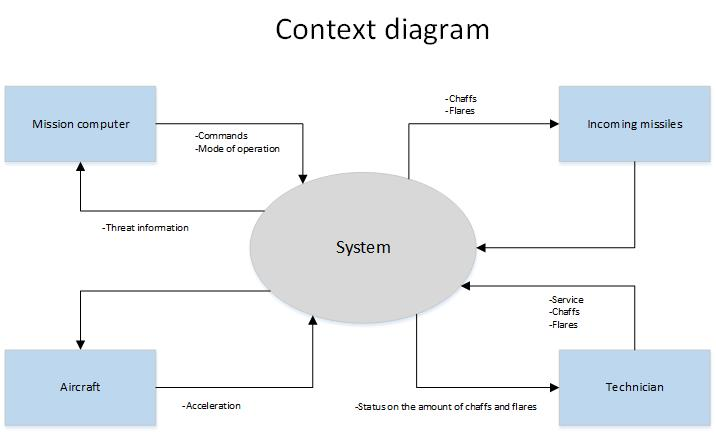
\includegraphics[scale=0.55]{./images/Systemoverview.jpg}
	\caption{Context diagram}
    \label{fig:Context diagram}
\end{figure}
\subsection{Document overview}
The purpose of this document is to specify the requirements for the system 'Self-protection suite for the F-16 combat aircraft'. The specified requirements throughout this document is legally in force in case of any uncertainties between Terma and The Royal Danish Air Force.
The document is composed of the the following main sections:


    \begin{description}
    \item[$\bullet$ Referenced documents:] Other documents that are referenced throughout this document is listed in this section.
    \item[$\bullet$ Requirements:] This is the main section that states all the requirements to the system.
    \item[$\bullet$ Quality provisions:] In this section methods for the verification of each requirement is specified.
 
    \end{description}

The content of this document is strictly confidential and is only supposed to be read by staff possessing the needed security clearance from either Terma or The Royal Danish Airforce. 
\section{System-wide design decisions}
System-wide design decisions for the system were made as part of the preliminary design effort. The team evaluated potential system-wide design issues and conducted analysis on how the system and its components would behave under different environmental conditions. 
TODO…. Write more stuff here

States of the system
The system will have different states depending on what is set by the mission computer. The system has three distinct states: 
•	Automatic: The system automatically detects and deploys the payload witouth the pilots interaction
•	Semi-automatic: The system detects the enemy missile but it asks for the pilots consent before deploying the payload
•	Manual: The pilot has to select the desired payload and deploy it himself.
Relevant constraints: The system has a built in safety feature which will prevent deployment of the payload when the plane is not airborne.
Detection and action upon incoming threats
We are using the missile warning system (MWS) to detect incoming missiles. Incoming missiles are considered an input in this design where the payload deployment system will respond to this input by deploying the payload if the missile is close enough to the aircraft. The payload is located in the pod that is mounted on the aircraft.

Components:
•	Pod
The physical dimensions of the pod cannot exceed 0.5X0.5X5 meter. The pod will have the same color as the rest of the aircraft in order to blend in with the environment. The pod will have a correct aerodynamic shape in such a way that it will create as little drag as possible so it will have minimum effect on the aircrafts speed. 
•	Cockpit unit
To prevent dispensing the payloads on the ground we will request sensor input from the mission computer that will make the system aware if the plane is in flight.
•	MWS
•	Dispenser
•	Magazines

After listing all the data. We justify that we use a cockpit unit that works with all of the data and acting on inputs from the missile warning system.

\section{System architectural design}
\input{./subfile/system_architectural_design.tex}
\subsection{System components}
\subsubsection{Component overview}
\begin{figure}[h]
\centering
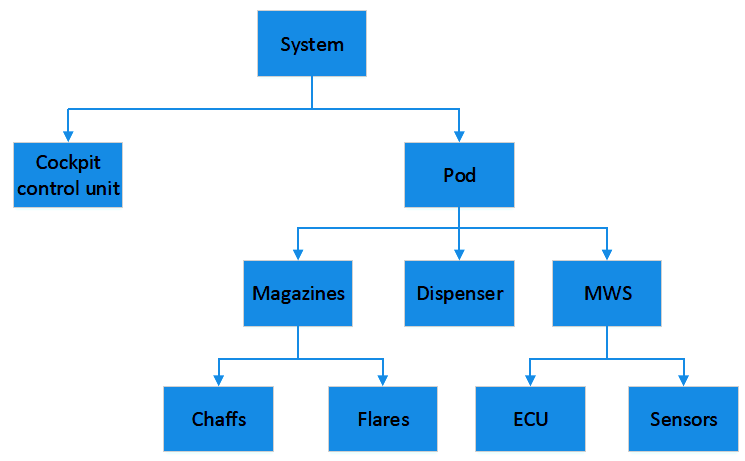
\includegraphics[scale=0.5]{./images/hierarchical.png}\\
\caption{Overview of components}
\label{fig:Component_overview}
\end{figure}

\begin{itemize}
\item Cockpit Control Unit (ID: CCU) 
\item Pod (ID: POD)
	\begin{itemize}
	\item Dispenser (ID: DIS)
	\item Magazines (ID: MAG)
	\end{itemize}
\end{itemize}
\begin{itemize}
\item MWS (ID: MWS)
	\begin{itemize}
	\item ECU (ID: ECU)
	\item Sensors (ID: SEN)
	\end{itemize}
\end{itemize}

\subsubsection{Detailed component description}
This section describes all system components and their connection to the requirements.

\paragraph{Cockpit Control Unit}\mbox{}\\
The Cockpit Control Unit (CCU) shall provide all necessary data to the aircraft mission computer.
\begin{itemize}
\item The CCU is responsible for switching between the three defined modes when receiving the respective signal from the aircraft mission computer (Req. No. 1-4).
\item The CCU shall be able to turn power ON and OFF for the dispensing system and the MWS (Req. No. 7).
\item The system shall be able to erase sensitive data upon input from a discrete zeroize signal from aircraft and the zeroize signal shall be received by the CCU (Req. No. 25-26).
\item The system shall provide the aircraft mission computer with status information and built-in test results (Req. No. 15).
\item The system status on individual LRU level shall be provided by cockpit unit (Req. No. 17).
\end{itemize}

\paragraph{POD}\mbox{}\\
The pod is a detachable compartment on an aircraft for carrying chaffs and flares. The pod also holds the dispenser, magazines and the MWS.
\begin{itemize}
\item The pod structure must be functional when exposed to steady state acceleration levels of 4g forward, 2.5g backward, 22g upward or 10g downward.
\item The weight of the pod cannot exceed 270 kg (Req. No. 28).
\item The pod shall be operational at temperatures of maximum 134 degree Celcius on outer skin and 152 degree Celcius on leading edge for maximum 3 minutes (Req. No. 29).
\item The pod shall be operational at temperatures of maximum 95 degrees Celcius on outer skin and 152 degrees Celcius on leading egde for a maximum of 25 minutes (Req. No. 41).
\item The physical dimensions of the pod cannot exceed 0.5$\times$0.5$\times$5 meter (Req. No. 35).
\end{itemize}

\paragraph{Dispenser}\mbox{}\\
The dispenser is the mechanism in which the magazines are installed.
\begin{itemize}
\item The dispenser shall be able to dispense forwards, downwards and sideways (Req. No. 6). 
\item The system shall be able to dispense a minimum of two payloads within 0.1 sec (Req. No. 8).
\item The system shall be able to dispense a pattern of payloads programmable by the customer (Req. No. 9).
\end{itemize}

\paragraph{Magazines}\mbox{}\\
The magazines contain the chaffs and flares.
\begin{itemize}
\item The pod shall include eight standard magazines (Req. No. 5).
\item The magasines shall be stored at no lower than -10 degrees Celcius and no higher than 70 degrees Celcius (Req. No. 26).
\end{itemize}

\paragraph{Chaffs and flares}\mbox{}\\
The chaffs and flares are the payload of the system. They are to be dispensed from the magazines.
\begin{itemize}
\item The aircraft has to be loaded with the payloads before takeoff (Req. No. 36).
\end{itemize}

\paragraph{Missile Warning System}\mbox{}\\
The missile warning system (MWS) consists of an Electronic Control Unit and six sensors.
\begin{itemize}
\item The aircraft has to be loaded with the payloads before takeoff (Req. No. 36).
\end{itemize}

\paragraph{Electronic Control Unit}\mbox{}\\
\begin{itemize}
\item The Electronic Control Unit (ECU) provides threat information in inertial format and the direction of the threat is relative to north (Req. No. 14).
\end{itemize}

\paragraph{Sensors}\mbox{}\\
The sensors are responsible for detecting incoming missiles (threats).
\subsection{Concept of execution}
subsection{Concept of execution}

This paragraph describes the concept of execution among the system components, which are shown in Figure.~{fig:Component_overview}. Since the relations between system 
components do not change dynamically, this section will describe the execution of a threat being detected.

\paragraph{Threat detected scenario}\mbox{}\\
This scenario unfolds when the sensors detect a missile threat. The sequence diagram shown below describes the automatic mode where the system responds without pilot 
interaction.

\begin{figure}[h]
	\centering
	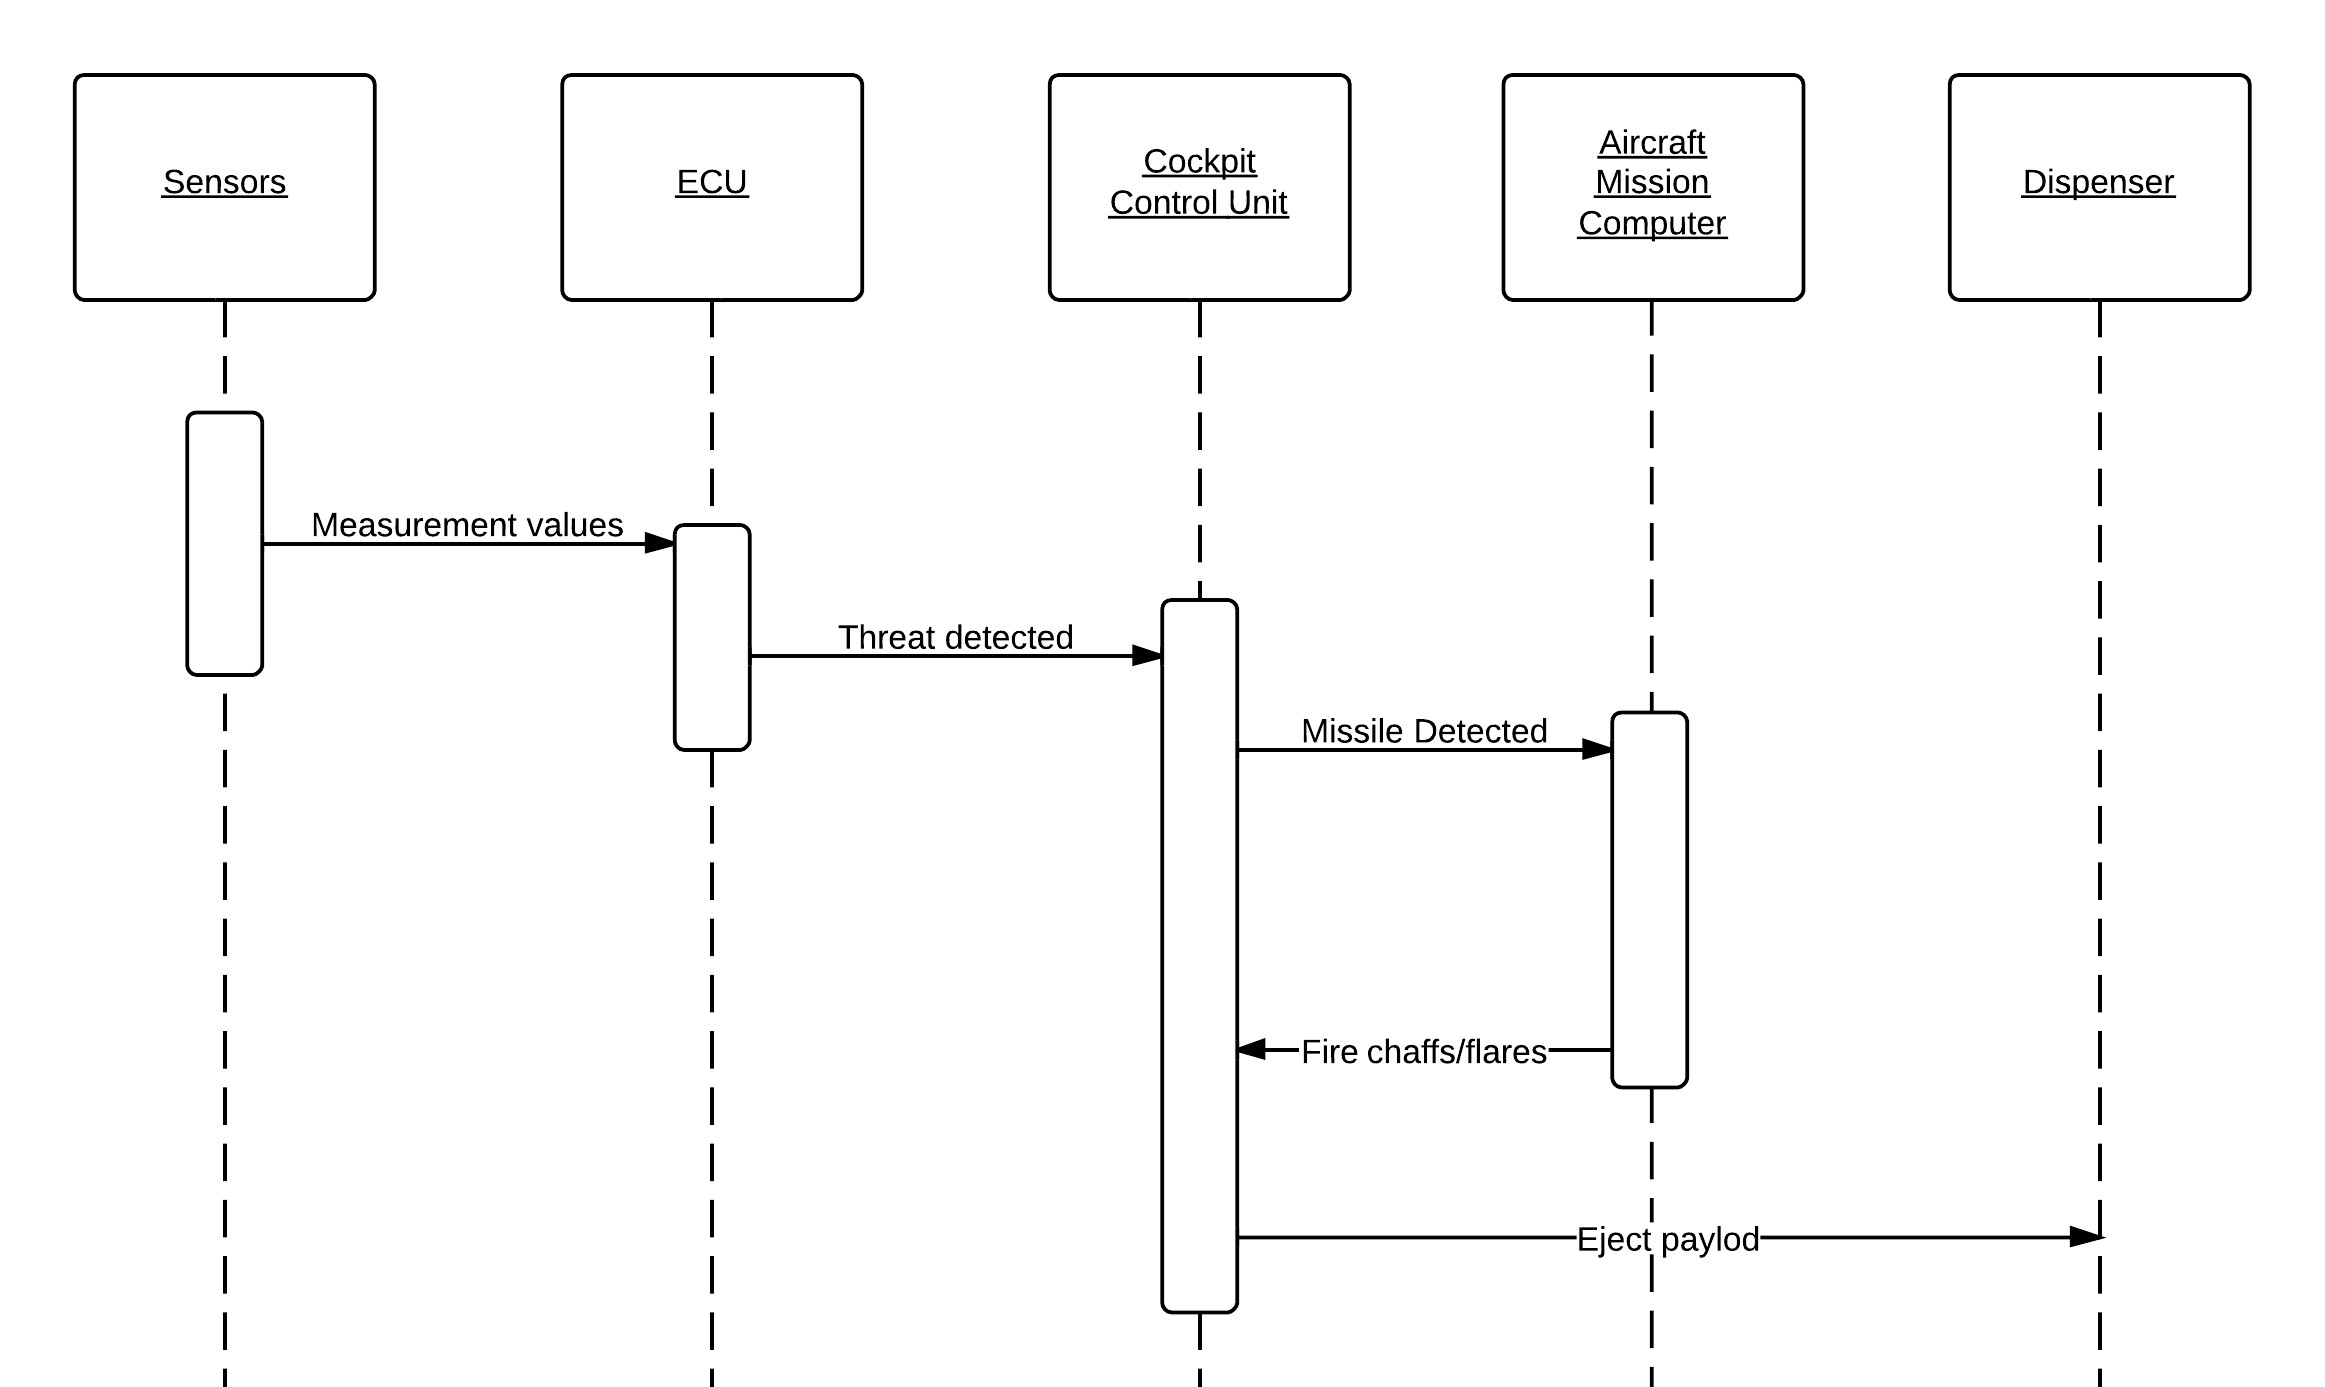
\includegraphics[scale=0.55]{./images/threatDetectedSequenceDiagram.png}\\
	\caption{Threat detected sequence diagram}
    \label{fig:threatDetectedSeqDia}
\end{figure}


\subsection{Interface design}
\subsubsection{External interfaces}

\subsubsection{Internal interfaces}

\begin{figure}[h]
	\centering
	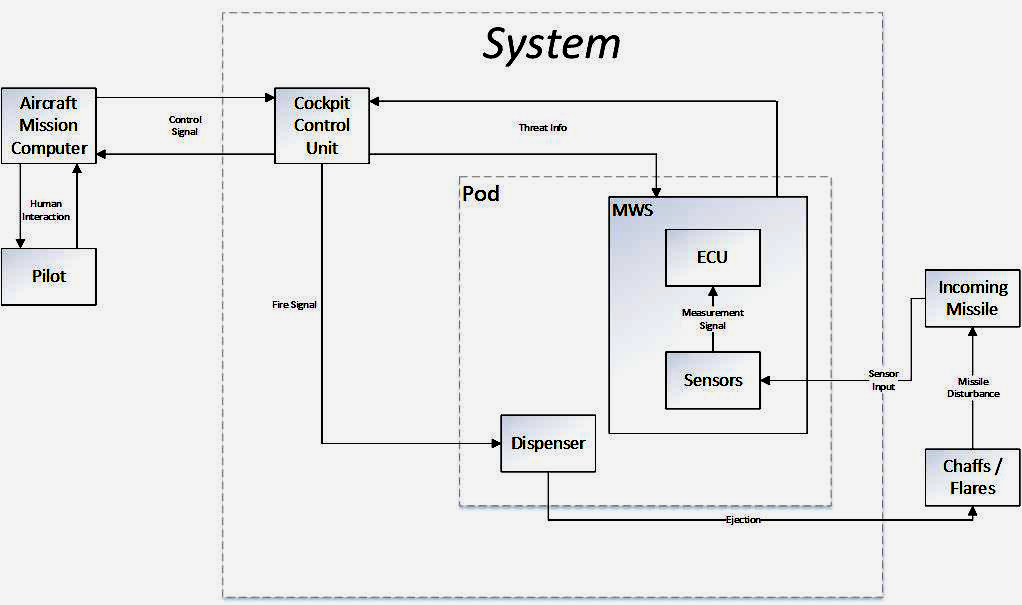
\includegraphics[scale=0.5]{./images/SignalFlowDiagram}\\
	\caption{Signal Flow Diagram}
    \label{fig:sigFlowDiagram}
\end{figure}
\section{Requirements traceability}
Every requirement has a test associated to it, e.g. "Req. No 1" is tested in the test "ReqNo1-T".
\end{document}
